%!TEX root = ../main.tex
\section{Introduction} 
\label{sec:intro}

%%%%%%%%%%%%%%%%%%%%%%%%%%%%%%%%%%%%%%%%%%%%%%%%%%%%%%

%%%%%%%%%%%%%%%%%%%%%%%%%%%%%%%%%%%%%%%%%%%%%%%%%%%%%%

% In real world, training a machine learning (ML) model over incomplete data with many missing values is a common scenario.
% Since it is well-known that \cc{incomplete} data may severely degrade the performance of ML models~\cite{cleaning4ml, chai2022data}, data-effective machine learning  (\aka data-centric AI~\cite{mlops}) has attracted much attention for obtaining high-quality train data to unlock the value of AI. 
% From another perspective, data-efficient ML is also widely considered to make the training proces more efficient. A commonly used strategy is to select a subset of train data (or coreset)~\cite{DBLP:journals/corr/abs-2011-09384,munteanu2018coresets} to represent the entire dataset such that ML models trained on the coreset can achieve similar performance to the ML models trained on the entire dataset.

% Apparently, users desire both data-effective ML (for training better ML models) and data-efficient ML (for saving training cost) when training over incomplete data, which is the focus of this paper.

Data-effective machine learning (ML) (\aka data-centric AI~\cite{mlops}) aims at obtaining high-quality training data to release the value of AI, because it is well-known that dirty data may severely degrade the performance of ML models~\cite{cleaning4ml, chai2022data}.

Data-efficient ML focuses on making the training process more efficient. A commonly used strategy is to select a core subset of training data (or coreset)~\cite{DBLP:journals/corr/abs-2011-09384,munteanu2018coresets} to represent the entire dataset such that ML models trained on the coreset can achieve similar performance to the ML models trained on the entire dataset.

Apparently, users desire both data-effective ML (for training better ML models) and data-efficient ML (for saving training cost). In this work, our main goal is to support both data-effective and data-efficient ML over \textit{incomplete data} where there are many missing values, which is very common in real-world scenarios~\cite{chai2022data, DBLP:conf/icml/YoonJS18, miao2022experimental}.


\begin{figure}
	\begin{minipage}{\columnwidth}\hspace{8em}
		\xymatrix @C=2pc @R=.5pc {
			&  
			& *+[F-:<3pt>]{\humanfunc(\train)} \ar[dr] 
			&  
			& *+[F-:<3pt>]{(1)~\corefunc(\humanfunc(\train))} 
			\\
			& *+[F-,]{\txt{Impute}} \ar[ur]^(.35){\txt{Human}} \ar[dr]_(.35){\txt{Auto}}
			&  
			& *+[F-,]{\txt{Coreset}} \ar[ur] \ar[dr]
			& 
			\\
			& 
			& *+[F-:<3pt>]{\autofunc(\train)} \ar[ur]
			&  
			& *+[F-:<3pt>]{(2)~\corefunc(\autofunc(\train))} 
			\\
			*+[F-:<3pt>]{\train} \ar[uur] \ar[ddr] 
			\ar@{.>}[rrrr]^{\txt{Data-effective $\ra$ Data-efficient}}_{\txt{Data-efficient $\ra$ Data-effective}}
			&
			& 
			& 
			&
			\\
			& 
			& 
			& 
			& *+[F-:<3pt>]{(3)~\humanfunc(\corefunc(D))} 
			\\
			& *+[F-,]{\txt{Coreset}} \ar[r]
			& *+[F-:<3pt>]{\corefunc(D)} \ar[r] 
			& *+[F-,]{\txt{Impute}} \ar[ur]^(.35){\txt{Human}} \ar[dr]_(.35){\txt{Auto}}
			& 
			\\
			& 
			& 
			& 
			& *+[F-:<3pt>]{(4)~\autofunc(\corefunc(D))} 
		}    
		\caption{Sequential methods.}
		\label{fig:sequential}
		\vspace{2ex}
	\end{minipage}
	%
	\begin{minipage}{\columnwidth}
		\begin{center}
			\begin{tabular}{|c|c|c|c|}
				\hline
				\textbf{Solution} & \textbf{Accuracy} & \textbf{Human Cost} & \textbf{Machine Cost} \\ \hline
				(1) $\corefunc(\humanfunc(\train))$	& High	& High	& Low	\\ \hline
				(2) $\corefunc(\autofunc(\train))$	& Low	& None	& Low	\\ \hline
				(3) $\humanfunc(\corefunc(D))$	& Low	& Low	& Low	\\ \hline
				(4) $\autofunc(\corefunc(D))$	& Low	& None	& Low	\\ \hline
				\rowcolor{black!10}
				Our goal	& High	& None or Low	& Low or Very Low	\\ \hline
				\rowcolor{black!10}
				(5) $\humanfunc(\goodfunc(\train))$	& High	& Low	& High 	\\ \hline
				\rowcolor{black!10}
				(6) $\autofunc(\goodfunc(\train))$	& Medium& None 	& High	\\ \hline
				\rowcolor{black!10}
				(7) $\goodfunc(\train,\circlearrowleft^\humanfunc)$	& High	& Low	& Low 	\\ \hline
				\rowcolor{black!10}
				(8) $\goodfunc(\train,\circlearrowleft^\autofunc)$	& Medium& None 	& Low	\\ \hline
				\rowcolor{black!10}	
				(9) $\goodfunc^+(\train,\circlearrowleft^\humanfunc)$	& High	& Low	& Very Low 	\\ \hline
				\rowcolor{black!10}
				(10) $\goodfunc^+(\train,\circlearrowleft^\autofunc)$	& Medium& None 	& Very Low	\\ \hline		
			\end{tabular}
		\end{center}
		\vspace{-1em}
		\caption{A comparison of different approaches (1--4: sequential methods; 5--10: our solutions).}
		\label{fig:comparison}
		\vspace{2ex}
	\end{minipage}
	\begin{minipage}{\columnwidth}
		\centering   
		\xymatrix @C=1.2pc @R=.5pc {\hspace{10em}
			&  
			& *+[F-:<3pt>]{(7)~\goodfunc(\train,\circlearrowleft^\humanfunc)}
			&  
			& *+[F-:<3pt>]{(5)~\humanfunc(\goodfunc(\train))} 
			\\
			*+[F-:<3pt>]{D} \ar[r] 
			& *+[F-,]{\txt{\ours}} \ar[r] \ar[ur]^(.35){\txt{Human$\circlearrowleft$}}  \ar[dr]_(.35){\txt{Auto$\circlearrowleft$}}
			& *+[F-:<3pt>]{\goodfunc(\train)}  \ar[r] 
			& *+[F-,]{\txt{Impute}}  \ar[ur]^(.35){\txt{Human}} \ar[dr]_(.35){\txt{Auto}}
			& 
			\\
			&  
			& *+[F-:<3pt>]{(8)~\goodfunc(\train,\circlearrowleft^\autofunc)}
			&  
			& *+[F-:<3pt>]{(6)~\autofunc(\goodfunc(\train))} 
		}    
		\caption{Our proposal and its variants.}
		\label{fig:ours}	
	\end{minipage}
\end{figure}


\stitle{Running data-effective and data-efficient tools sequentially.} Intuitively, we can either run data imputation methods first for data-effective and then run coreset selection algorithms denoted by $\corefunc(\cdot)$ for data-efficient, or vice versa.
%
Moreover, for data-effective solutions through data cleaning, we generally consider two cases, either human-based solutions denoted by $\humanfunc(\cdot)$ or automatic solutions denoted by $\autofunc(\cdot)$. 
%
In summary, we have the following four cases, as shown in Figure~\ref{fig:sequential}:


\stab
\textit{$\bullet$ First data-effective (impute) then data-efficient (coreset):}

\bi
	\item[(1)] Impute-Human: $\humanfunc(\train)$ $\ra$ Coreset:  $\corefunc(\humanfunc(\train))$
	\item[(2)] Impute-Auto: $\autofunc(\train)$ $\ra$ Coreset: $\corefunc(\autofunc(\train))$
\ei

\stab
\textit{$\bullet$ First data-efficient (coreset) then data-effective (impute):}

\bi
	\item[(3)] Coreset: $\corefunc(\train)$ $\ra$ Impute-Human: $\humanfunc(\corefunc(D))$
	\item[(4)] Coreset: $\corefunc(\train)$ $\ra$ Auto-Human: $\autofunc(\corefunc(D))$  
\ei

Next let's discuss the pros and cons of the above approaches. 

Case (1) has high human cost, low machine cost, and high accuracy in terms of the trained ML models.
%
Case (2) has zero human cost, low machine cost, but with low accuracy because automatic imputation may not be good enough.
%
Case (3) has low human cost, low machine cost, but with low accuracy because corset selection over a dirty dataset may not ensure to compute a ``good'' coreset. 
%
Case (4) has no human cast, low machine cost, but with low accuracy with the similar reason as  (3).
%
The comparison of the above four methods can be found in Figure~\ref{fig:comparison}.


\stitle{Our goal.} Clearly, a primary goal is to achieve high accuracy for ML models, where only case (1) can achieve. 
Case (2) achieves low accuracy because automatic imputation is hard to be accurate.
The main obstacle for making (1) practical is its high human cost. 
Hence, our \textit{main goal} is to achieve high accuracy with no or low human cost, and with low machine cost.

Consider cases (3) and (4), the main reason for them to achieve low accuracy is because they cannot compute a good coreset directly from the dirty data. Intuitively, if we can compute a good coreset directly from the dirty data, we can cheaply clean the coreset to achieve high accuracy, where the ``goodness'' means that the subset of tuples selected from the dirty data is similar to the subset of tuples selected from the clean data.

\stitle{Challenge.}
The main challenge of computing a good coreset from dirty data is to accurately estimate the ground truth of each missing value; otherwise, we cannot select a coreset to well represent the clean data. This is a known hard problem because each missing value may have multiple possible repairs. Also, because a coreset selection algorithm is typically iterative that each tuple is selected per iteration~\cite{DBLP:conf/icml/MirzasoleimanBL20}, selecting a bad tuple may cause cascade amplification to the following iterations, resulting in a bad coreset.


\stitle{Our proposal.}
To tackle the above challenge, we model the combinations of possible repairs as possible worlds of the original dirty data $D$. 
We then formulate it as an optimization problem for selecting an expected optimal coreset that can represent the  possible worlds of $D$ via gradient approximation without training in advance. We prove this problem to be NP-hard. We propose an approximate algorithm, called \ours, denoted by $\goodfunc(\cdot)$, with the main idea to iteratively add a tuple with the highest utility  into the coreset. 
After a good coreset is computed, we can either use human imputation or automatic imputation to impute the data, as shown in Figure~\ref{fig:ours}.
We further elaborate these two methods below:

\bi
	\item[(5)] \ours: $\goodfunc(D)$ $\ra$ Impute-Human: $\humanfunc(\goodfunc(D))$
	\item[(6)] \ours: $\goodfunc(D)$ $\ra$ Impute-Auto: $\autofunc(\goodfunc(D))$
\ei

However, one main drawback is that modeling possible worlds of $D$ is computationally expensive, which hinders the practicability of the \ours algorithm.  To address this high computational cost problem, we further propose  imputation-in-the-loop optimization (with either humans or automatic methods) into the \ours algorithm (see methods 7 and 8 in Figure~\ref{fig:ours}). To this end, the optimized algorithms can significantly reduce the number of possible worlds, thus achieving low computational cost. 

\bi
	\item[(7)] \ours with human-in-the-loop imputation: $\goodfunc(D, \circlearrowleft^\humanfunc)$ 
	\item[(8)] \ours with machine-in-the-loop imputation: $\goodfunc(D, \circlearrowleft^\autofunc)$
\ei






Besides, since the above methods for coreset selection incorporate at least one iteration over the entire dataset, it is not very efficient when the dataset is large, so we propose a group-based acceleration strategy to further reduce the machine cost. The key idea is to assign similar tuples in $D$ into a group, and thus the coreset is selected to represent these groups. Since the groups can still represent the distribution of $D$, the selected coreset is still well-performed. In this way, we only need to iterate these groups, with a much smaller number than the tuples of $D$, and thus the efficiency is improved. We also provide a theoretical analysis with respect to the group-based strategy. Hence, we further have the following 2 methods.

\bi
\item[(9)] Group-based \ours (\texttt{GoodCore}$^+$) with human-in-the-loop imputation: $\goodfunc^+(D, \circlearrowleft^\humanfunc)$.
\item[(10)] \texttt{GoodCore}$^+$ with machine-in-the-loop imputation: $\goodfunc^+(D, \circlearrowleft^\autofunc)$.
\ei

A comparison of methods (5)--(10) is given in Figure~\ref{fig:comparison}. Note that method (10) is likely to be a good choice because it can achieve a high ML accuracy with low human cost and low machine cost.
%


\stitle{Contributions}
We make the following contributions.

\be
	\item[(i)] \textit{Two birds with one stone.} 
	We study the problem of solving both data-effective and data-efficient ML in one framework, which is an important but not addressed problem.
 	(Section~\ref{sec:overview})

 	\item[(ii)] \textit{NP-hardness and approximate solutions.}
	We prove the NP-hardness of the problem. We propose a greedy algorithm with an approximate ratio. 
	(Section~\ref{sec:without})

	\item[(iii)] \textit{Imputation-in-the-loop optimizations.}
	We develop optimization techniques that integrate imputation-in-the-loop into the coreset selection process, to improve the efficiency while achieving high accuracy. We also analyze the convergence rate of our method and theoretically prove that it can converge fast. 
	(Section~\ref{sec:human})
	
	\item[(iv)] \textit{Group-based acceleration.}
	We develop group-based techniques to further improve the efficiency. We also analyze the theoretical guarantee and convergence of the proposed techniques. 
	(Section~\ref{sec:group})


	%\item[(iv)] \textit{Convergence rate analysis.}\nan{Add this section as a contribution. Otherwise, the reviewers may not even know you have this section.}

	\item[(v)] \textit{Experiments.}
	We conduct extensive experiment on 8 real-world datasets and compare with 10 baselines to show that \ours can select a well-performed coreset to achieve both data-effective and data-efficient ML while consuming a low human cost. 
	(Section~\ref{sec:exp})
\ee

% An intuitive strategy is to first make the data ``effective'' through data cleaning, and then make the data ``efficient'' by selecting a coreset.
% If we further consider automatic cleaning or human cleaning, we have two solutions as shown in Figure~\ref{fig:solutions}.


% \bi
% 	\item[(1)] Auto-Impute $\ra$ Coreset ($C^A$): First run automatic data imputation methods, and then run coreset selection algorithm. 
% 	\item[(2)] Human-Impute $\ra$ Coreset ($C^H$): First use manual imputation methods, and then run coreset selection algorithm. 
% \ei




% %%%%%%%%%%%%%%%%%%%%%%%%%%%%%%%%%%%%%%%%%%%%%%%%%%%%%%
% \begin{figure}[!t]
% 	\xymatrix @C=2.5pc @R=.5pc {
% 	&  
% 	& *+[F-:<3pt>]{D^A} \ar[dr] 
% 	&  
% 	& *+[F-:<3pt>]{(1)~C^A} \ar@{.>}[dd]_{\txt{$<$}}
% 	\\
% 	*+[F-:<3pt>]{D} \ar[r] \ar[dddr]
% 	& *+[F-,]{\txt{Impute}} \ar[ur]^{\txt{Auto}} \ar[dr]_{\txt{Human}}
% 	&  
% 	& *+[F-,]{\txt{Coreset}} \ar[ur] \ar[dr]
% 	& 
% 	\\
% 	& 
% 	& *+[F-:<3pt>]{D^H} \ar[ur]
% 	&  
% 	& *+[F-:<3pt>]{(2)~C^H} 
% 	\\
% 	&
% 	&
% 	& *+[F-:<3pt>]{(4)~C_G^H} \ar@{.>}[ur]^\approx
% 	&
% 	\\
% 	& *+[F-,]{\txt{\ours}} \ar[r]
% 	& *+[F-:<3pt>]{C_G} \ar[ur]^{\txt{Human}} \ar[dr]_{\txt{Auto}}
% 	& 
% 	& 
% 	\\
% 	&
% 	&
% 	& *+[F-:<3pt>]{(3)~C_G^A} \ar@{.>}@/_4pc/[uuuuur]^{\txt{$>$}} \ar@{.>}[uuur]^{\txt{$<$}}
% 	& 
% 	}    
%    	\caption{}
%    \label{fig:solutions}
% \end{figure}
% %%%%%%%%%%%%%%%%%%%%%%%%%%%%%%%%%%%%%%%%%%%%%%%%%%%%%%

% \bi
% %	\item Data-effective ML requires high-quality data
% %	\item Data-efficient ML aims at reducing training cost
% %	\item In this work, we tackle the problem of data-effective and data-efficient ML over incomplete data, which is very common in practice
% 	% \item If we impute data first, and then compute the coreset
% 	% \bi
% 	% 	\item[1.] AutoImpute $\ra$ Coreset (Efficient but Ineffective)
% 	% 	\item[2.] HumanImpute $\ra$ Coreset (Inefficient but Effective)
% 	% \ei
% 	%\item In order to achieve both data-efficient and data-effective, we propose to compute a ``good'' coreset.

% 	%{\bf Problem Challenges of computing a good coreset directly from dirty data.}
% 	%Essential challenge: ``Guess'' the ground truth. In practice, we don't know the ground truth, so we can only compute an expectation ...

% %	{\bf Our proposal.} Enumerate possible worlds. Iteratively select one tuple with the highest expected utility to be added to the coreset.

% 	\bi
% 		\item[3.] CleanCore $\ra$ HumanImpute (Efficient and Effective) High machine cost, low human cost
% 		\item[4.] CleanCore $\ra$ AutoImpute (Efficient but Ineffective)
% 		High machine cost, zero human cost
% 	\ei
% 	\item {\bf Optimizations.} The computational cost of Cleancore is still high because .... To further optimize xxx, we also propose optimized algorithm that directly outputs imputed coreset 
% 	\bi
% 		\item[5.] CleanCore$^{Human}$ Low machine cost, low human cost, high effectiveness
% 		\item[6.] CleanCore$^{Auto}$
% 	\ei
% 	Please refer to Table~\ref{} for the pros and cons of methods (1)--(6). 
% \ei


%In the era of machine learning (ML), data-effective ML is to require high-quality data (\eg data cleaning) for training a well-performed model.  Given train data, data-efficient ML aims at reducing training cost without influencing the  model accuracy.  Recently, there are many efforts~\cite{} on computing a subset of the full train dataset, \aka \textit{coreset}, that can achieve efficient training without sacrificing much the accuracy theoretically and practically. Putting them together, in this work, we tackle the problem of data-effective and data-efficient ML over incomplete data, which is very common in practice caused by reasons ranging from software bugs, unreliable sensor readings to human errors~\cite{}.


%\noindent \textbf{Coreset in Machine Learning.} Given train data, data-efficient machine learning  aims to train ML models more efficient without sacrificing the model accuracy. To improve the efficiency, typical methods like stochastic gradient decent~\cite{} focus on judiciously accelerating the training algorithm. Besides, recently there are many efforts~\cite{} on computing a subset of the full train dataset, \aka \textit{coreset}, that can achieve efficient training without sacrificing much the accuracy theoretically and practically.


%\noindent \textbf{Incomplete data.} However,  real-world datasets are always dirty, making the selected coreset also dirty, which degrades the model performance. Among different types of data errors, incomplete data caused by missing values is a serious problem that a data scientist often has to solve. Incomplete data arises for different common reasons ranging from software bugs, unreliable sensor readings to human errors~\cite{}. More importantly, different from other errors (\eg unnormalized values, duplicated records, inconsistency) that can sometimes be remained as they are, incomplete data must be tackled (deleted or imputed) first for ML training.



%Hence, in this paper, we aim to solve the problem of \textit{how to select a  coreset that can still achieve good performance when there exist incomplete tuples in the train dataset.}



%\noindent \textbf{Possible solutions.}   Given an incomplete train dataset ($D$), to tackle this problem, there are some intuitive possible solutions. Let us first introduce them  (Figure~\ref{fig:coresets}), analyze their benefits and limitations. 


%\noindent \underline{[1.\textit{Auto-impute $D$ $\rightarrow$ Coreset selection.}]}
%This solution automatically imputes $D$, derives $D^A$, selects the coreset $C^A$ and trains on $C^A$, as shown in Solution (1), which is efficient because $C^A$ is much smaller than $D^A$. However, the model accuracy is not good because automatic  methods cannot always  guarantee that $D^A$ is close to the ground truth. Naturally, based on  $D^A$, the coreset $C^A$ is also not good enough. In short, solution (1) is efficient but not effective enough.


%\noindent \underline{[1.\textit{Auto-impute $\train$}]} is an straightforward solution (Solution \ding{202}) that  imputes the missing values using  automatic approaches (based on the data statistics or learned distribution), and then train the model on the dataset after imputation, but the training efficiency is low due to it is trained on the full data (use 23 minutes for imputation and training as shown in Figure~\ref{fig:mot_exp}). Also, the accuracy (0.671) is just medium because automatic  methods cannot always be accurate. 

%\noindent \underline{[2.\textit{Human-impute $D$ $\rightarrow$ Coreset selection.}]} 
% To improve the effectiveness,  as shown in Solution (1), we can rely on human to impute $D$ as $D^H$, and compute the coreset $C^H$. Because of the human intelligence,  $D^H$ is likely to be  close to the ground truth, and thus $C^H$  performs better than $C^A$. However, the human cost is prohibitively expensive when there are many missing values. To summarize, solution (2) is effective but not efficient.



%\begin{example}\label{example:motexp}
%	\add{As shown in Figure~\ref{fig:mot_exp}, we implement Solution~\ding{202} and~\ding{203} on a real-world dataset, which contains 12500 incomplete tuples and 20000 complete tuples. We can see that both Solution~\ding{202} and~\ding{203} can improve the performance of the model than directly training a model on the dirty dataset $\train$ (with an accuracy of 0.612). Although Solution~\ding{202} can achieve a high accuracy 0.716, the human cost (12500 \cc{tuples}) is too expensive. We can see that Solution~\ding{203}  reduces the human cost (\ie 174), but the accuracy decreases to 0.655 because automatic approaches are not accurate enough.} 
%\end{example}




%Fortunately, we can try  data-efficient coreset-based solutions to alleviate these issues. Two intuitive solutions are as follows.  

%\noindent \underline{[3.\textit{Auto-impute $\train$ $\rightarrow$ Coreset selection.}]} This solution automatically imputes $\train$, selects the coreset and trains on the much smaller coreset (Solution \ding{204}). \cc{Although it has high efficiency (4.6 minutes), the accuracy (0.649) is low because the automatic methods may not generalize well and the coreset also sacrifices some accuracy.}

%\noindent \underline{[4.\textit{Auto-impute $\train$ $\rightarrow$ Coreset selection $\rightarrow$ Human verification.}]} Based on the coreset computed by the last solution, this solution involves human to verify the tuples in the coreset that are imputed by automatic methods (Solution \ding{205}), the accuracy (0.655) can be improved but still not high. The reason is still that  automatic methods cannot achieve much accurate imputation of $\train$, based on which the selected coreset is also not good enough.




%\noindent \textbf{Possible solutions.} Given an incomplete train dataset ($\train$) with missing values, an intuitive solution is to first impute all the values (producing $\trainc$), conduct the coreset selection, and then derive the coreset $\core^*$. Hopefully, training on $\core^*$ can get competitive performance of training on $\trainc$. To ensure  a high-quality imputation, some recent  works~\cite{} rely on humans to impute  the data, which can lead to an accurate $\trainc$. However, human is not free,  which is prohibitively expensive when there are many missing values, as shown in Figure~\ref{fig:coresets}-Solution \ding{202}. Alternatively, as shown in Figure~\ref{fig:coresets}-Solution \ding{203}, we can also leverage some automatic approaches~\cite{} (based on the data statistics or learned distribution) to impute the missing values, compute the coreset and ask the human to further verify the coreset. Although it costs less, but it cannot achieve high accuracy  because the selected  $\core'$ is not a good coreset.  The reason is that these automatic imputation methods cannot always be accurate because the learned or statistical knowledge may not generalize well, and thus$\core'$ is computed based on a relatively dirty dataset (\ie clearly $\core' \neq \core^*$). Hence, training on $\core'$  is not equivalent of training on $\trainc$.
 
 
%\begin{figure*}[!t]
%	\centering
%	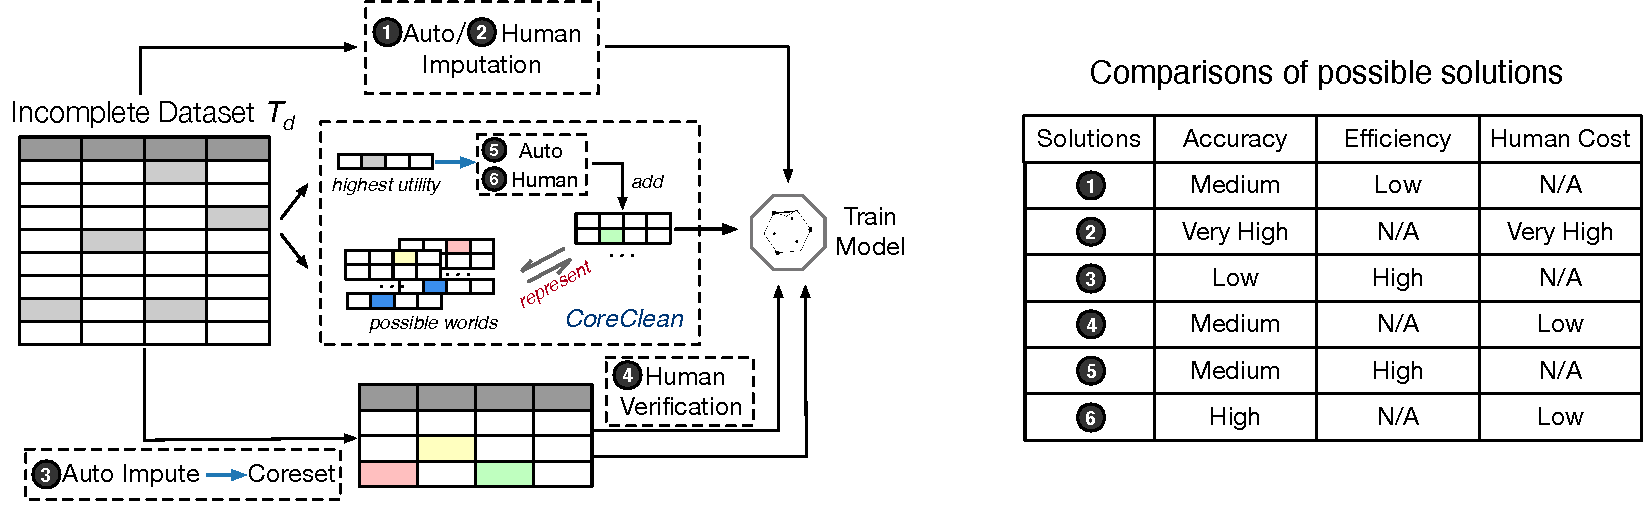
\includegraphics[width=1\textwidth]{figs/solutions}
%	\vspace{-3.2em}	
%	\caption{Possible solutions and \ours.}
	%\label{fig:coresets}
%\end{figure*}



%Hence, in this paper, we aim to solve the problem of \textit{how to select a good coreset that can achieve good performance when there exist incomplete tuples in the train dataset.}

%\add{Example~\ref{example:motexp} tells us that involving human into data cleaning can improve the accuracy. However, high human cost is unacceptable. Thus, introducing automatic data cleaning methods can significantly reduce the human cost.}

%\noindent \textbf{Key challenge.} As discussed, the above  intuitive solutions cannot achieve a good trade-off between data effectiveness and data efficiency. The essential challenge of  selecting a good coreset over incomplete data is that it is hard to know the ground truth of $D$, and thus the selected coreset is hard to represent the accurate complete version of $D$.

%To summarize, the key of coreset selection with incomplete data is to select a good coreset as a representative of the fully imputed train dataset. But unfortunately, $\trainc$ is rather hard to obtain  because of  two challenges. (1) There are many missing values (each  has several possible imputation choices) in $\train$, which constitute a large number  of possible worlds as candidates of $\trainc$. Hence, it is hard for an automatic method to accurately select one as $\trainc$ among these possible worlds . (2) Although we can hire  humans to accurately impute each value, it will introduce high cost. 

 

% \noindent \textbf{Our proposal.} 
% To address the challenge, we propose \ours that can select a well-performed coreset over incomplete data effectively and efficiently. 
% As discussed above, although we cannot get the ground truth in advance, \ours will select an informative coreset $C_C$ considering  the possible worlds of $D$. Overall, We formulate it as an optimization problem for selecting an expected optimal coreset that can represent the  possible worlds of $D$. We prove that this problem is NP-hard. We propose an approximate algorithm, with the main idea that greedily adds tuple with the highest utility  into the coreset. To be specific,  a tuple with a higher utility indicates that including the tuple can make the coreset better represent the possible worlds. Afterwards, $C_C$ can be imputed by automatic methods or human, and we can get $C_C^H$ and $C_C^A$ as shown in solution (3) and (4) respectively. To summarize, since $C_C$ is a good coreset, solution (3) can achieve a higher accuracy than solution (1), and solution (4) is competitive with solution (2) but with a much lower human cost.  
% %But the full data at hand $(\train)$ is incomplete, so  the utility is computed to measure whether the tuple can make the coreset well represent the possible worlds of $\train$.

% \noindent \textbf{Optimizations.} However, since the number of possible worlds of $D$ is extremely large because of there may exist many missing values in $D$, the computational cost of \ours is high. To address this,  we further propose imputation-in-the-loop strategies that  leverage automatic methods (solution (5)) or human (solution (6)) to impute the tuples in the coreset, once one or a small batch of incomplete tuples are added, which can greatly reduce the number of possible worlds. 	Please refer to Table~\ref{tab:compare} for the advantages and disadvantages of solutions (1)-(6). 


% \begin{table}[]
% 	\caption{Comparisons among possible solutions}\label{tab:compare}
% 	\begin{tabular}{|c|c|c|c|}
% 		\hline
% 		\multicolumn{1}{|l|}{Solution} & \multicolumn{1}{l|}{Accuracy} & \multicolumn{1}{l|}{Human Cost} & \multicolumn{1}{l|}{Machine Cost} \\ \hline
% 		(1)                            & Low                           & 0                               & Low                               \\ \hline
% 		(2)                            & High                          & High                            & Low                               \\ \hline
% 		(3)                            & Medium                        & 0                               & High                              \\ \hline
% 		(4)                            & High                          & Low                             & High                              \\ \hline
% 		(5)                            & Medium                        & 0                               & Low                               \\ \hline
% 		(6)                            & High                          & Low                             & Low                               \\ \hline
% 	\end{tabular}
% \end{table}

%There are many advantages. First, the number of possible worlds can be greatly reduced after some tuples are imputed,  and thereby the efficiency can be improved. Second, human is more accurate, so the human-in-the-loop strategy can help continuously improve the coreset quality. Third, since we just need to impute the incomplete tuples in the coreset, which is much smaller than $\train$, the cost is also greatly reduced.
 
 %\add{As shown in Figure~\ref{fig:mot_exp},  our Solution~\ding{204} can significantly reduce the human cost from 12500 to 153 without sacrificing the accuracy much \cc{(0.706)}.}


%\begin{figure}
%	\centering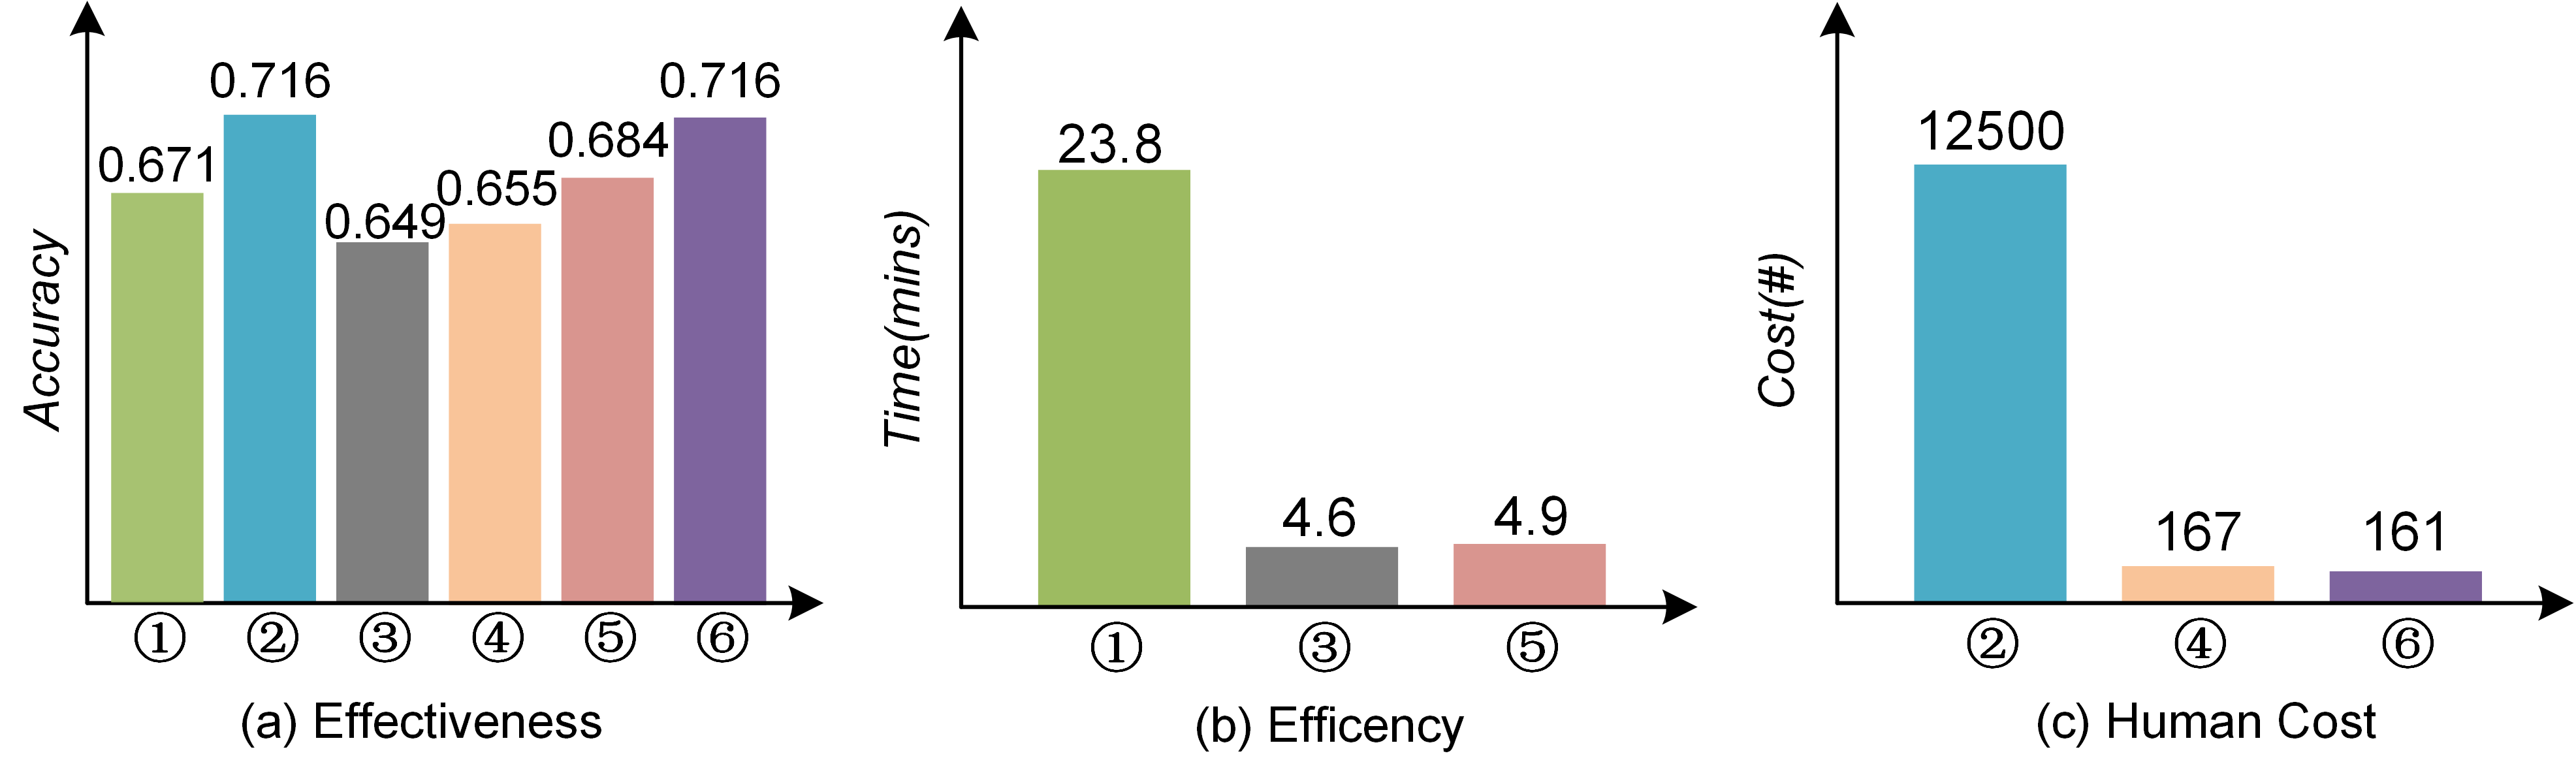
\includegraphics[width=\columnwidth]{figs/mot_exp.png}
%	\vspace{-1em}
%	\caption{Comparison with possible solutions and \ours.}
%	\label{fig:mot_exp}
%\end{figure}




 %and thus  tuples  are selected from the $\train$ iteratively and added into the coreset incrementally. To ensure the accuracy, we ask the humans to impute the selected tuples  iteratively such that  the  quality of the  selected tuples can be improved continuously in further iterations. Since we just leverage the human to impute the tuples within the selected coreset, the cost if greatly reduced (for \textbf{C2}).

% To summarize, we make the following contributions.

% \noindent (1) To the best of our knowledge, we are the first to study  coreset selection for supervised ML with incomplete data, and  formally define the problem (Section~\ref{sec:pre}). 

% \noindent (2) We prove the hardness of the problem. To solve the problem, we  propose a greedy algorithm with an approximate ratio using a single human iteration (Section~\ref{sec:without}). 

 
% \noindent (3) We further develop an imputation-in-the-loop strategy that   iteratively imputes one  or a small batch of tuple(s) during the coreset selection (Section~\ref{sec:human}).

% \noindent (4) We conduct extensive experiment on XX real-world datasets to show that \ours can select a well-performed coreset \cc{XX} while consuming a low human cost \cc{XX} (Section~\ref{sec:exp}).

% expected coreset- Np hard

% human in the loop

% In iterations, each iteration, incrementally select batch, ask human to impute, continuously improve the accuracy.


%automatically select a coreset $\core$ that is expected to be  optimal, and then impute the missing values among the small coreset by humans with a low cost, as shown in Figure~\ref{fig:coresets}-Solution \ding{204}.

%There are a multitude of reasons why they occur: ranging from human errors during data entry, incorrect sensor readings, to software bugs in data science pipelines [16]. Moreover, different from other types of errors (e.g., wrong names/addresses, unnormalized values, and violations of integrity constraints) that sometimes can be remained as they are, for ML modeling, these missing data fields must be deleted or imputed first.

%For many machine learning (ML) projects, the main bottleneck is the lack of high-quality train data, so as to produce high-quality ML model. However,  data collection or acquisition from various real-world datasets always incorporates errors in the train data such as missing values, outliers, inconsistency, etc, which may highly affect the model performance~\cite{}. Hence, it is indispensable to clean the data with the goal of improving the model.







%-- statistic-based, generative model-based, DL-based, but they are not accurate enough






